%\documentclass[11pt,fleqn]{article}
%\begin{document}
%
%\end{document}


\labday{Tuesday, 16 February 2016}

\experiment{DC Circuit Measurements}

\subexperiment{Introduction}
In this Experiment the voltages across a DC-Circuit (as shown in Fig. \ref{fig:DC}) shall be calculated and then measured with.

\subexperiment{Procedure}

\begin{figure}[H] % Example of including images
\begin{center}
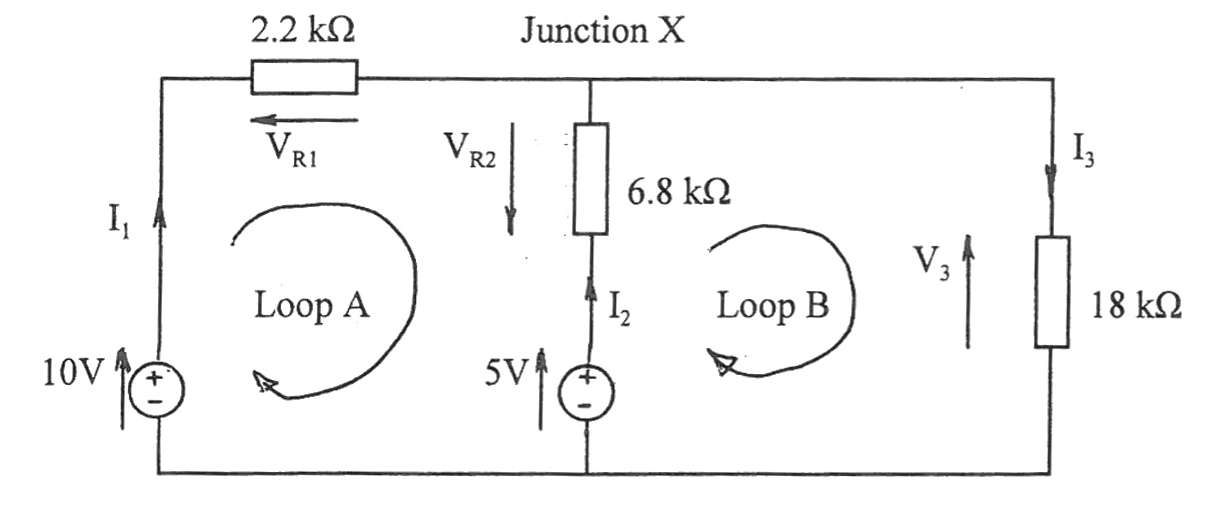
\includegraphics[width=1\linewidth]{LabOne/Exp1}
\end{center}
\caption{DC Measurement Setup}
\label{fig:DC}
\end{figure}


\begin{enumerate}
  \item Switch on all the instruments you intend to use. They take time to warm up and reach a stable performance
  \item Select the resistors that you need for the circuit. Note in your log book the colour code on each and the value. The details of the colour code is on the top of the resistor box and is also in any ELFA, RS or Farnell Catalogue.
\item Connect up the circuit shown in Fig. \ref{fig:DC} , dc on the bread board with long wires for the power supplies.
\item Set the dual power supply to ‘independent outputs’ with 10 Volts on one output and 5 Volts on the other. Connect these to your circuit. Check that the current limits are set working and set them to suitable values.
\item Check that the voltmeter is Switched to do measurements and use it to measure all the
voltages in the circuit. That is both dc supply voltages and the voltages across the resistors,
V$_{RI}$, V$_{R2}$ and V$_3$. Record the values in the log book.
\item Use the oscilloscope to measure the voltages that were measured in 4 above. Again record
these. 

Note the oscilloscope measures with reference to ground or zero volts. You can use the
difference function on the oscilloscope to find the voltages across R1 and R2. Connect one
input probe at one end of the resistor and the other probe at the other end. Then switch the
display to the difference by: \\
i Press the plusminus key between the inputs. \\
ii Turn Function 1 ON using the left hand key below the display. \\
iii Press the Function 1 menu key. \\
iv press the selection key to give 1-2.
The display should now give the difference between the two inputs. Whether the result is
positive or negative depends on which end of the resistor you connected each probe.

\end{enumerate}




%\lipsum[1]

\subexperiment{Results}
Selecting resistors:
\begin{table}[h]
\centering
\caption{Chosen Resistance}
\label{tab:Resistance}
\begin{tabular}{ll}
\textbf{Resistance} & \textbf{Color Code} \\
2.2 k$\Omega$ &  Red Red Black Brown Brown \\
6.8 k$\Omega$ &  Blue Gold Black Brown Brown\\
18 k$\Omega$ &  Brown Gray Blue Red Brown                 
\end{tabular}
\end{table}
All Resistances were checked with a voltmeter after choosing the appropriate resistor. The 18 k$\Omega$ resistor was slightly off the expected value, with a value of 17.78 k$\Omega$.
%\begin{itemize}
%  \item 2.2kOhm, Color Code: 
%  \item 6.8kOhm, Color Code: 
%  \item 18.0kOhm, Color Code:  (checked with Voltmeter: 17.78Ohm)
%\end{itemize}
\newline
After setting the current limits the voltage of the two channels of the Power Supply were set to 9.94V and 5.04V.

Then the voltages at the Resistors were measured using an ordinary Multimeter (cf. Table \ref{tab:ResistanceDC1}).

\begin{table}[h]
\centering
\caption{Voltage Drop measured with Voltmeter in DC-Circuit}
\label{tab:ResistanceDC1}
\begin{tabular}{ll}
\textbf{Resistance} & \textbf{Measured Voltage Drop} \\
R$_1$ = 2.2 k$\Omega$ &  V$_{R1}$ = 1.94 V \\
R$_2$ = 6.8 k$\Omega$ &  V$_{R2}$ = 2.975 V\\
R$_3$ = 18 k$\Omega$ &  V$_3$ = 8.00 V                
\end{tabular}
\end{table}



Now the dropped voltage across the resistors is measured again, by using an oscilloscope with two probes, one connected before the appropriate resistor and the other after the resistor. By subtracting the measured values we obtain the dropped voltage (cf. Table \ref{tab:ResistanceDC2}). This Measurement is only done for R$_1$ and R$_2$, as requested in the procedure.

\begin{table}[h]
\centering
\caption{Voltage Drop measured with Oscilloscope in DC-Circuit}
\label{tab:ResistanceDC2}
\begin{tabular}{ll}
\textbf{Resistance} & \textbf{Measured Voltage Drop} \\
R$_1$ = 2.2 k$\Omega$ &  V$_{R1}$ = 1.6347 V \\
R$_2$ = 6.8 k$\Omega$ &  V$_{R2}$ = 3.015 V            
\end{tabular}
\end{table}


\subexperiment{Summary}






%-----------------------------------------

\experiment{AC Circuit Measurement}

\subexperiment{Introduction}

\subexperiment{Procedure}


\begin{figure}[H] % Example of including images
\begin{center}
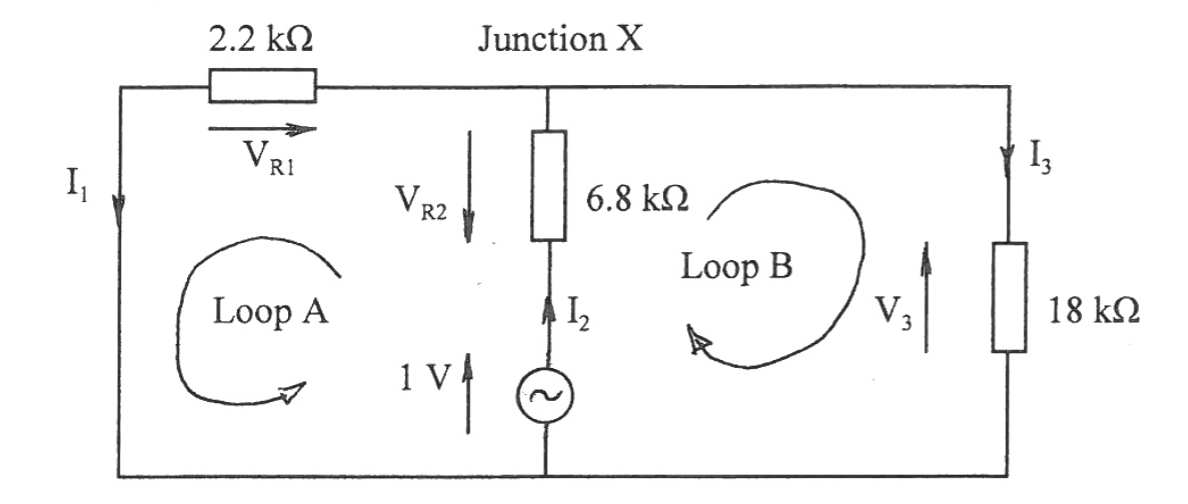
\includegraphics[width=1\linewidth]{LabOne/Exp2}
\end{center}
\caption{AC Measurement Setup}
\label{fig:AC}
\end{figure}

\begin{enumerate}
  \item Modify the circuit on the bread board to that shown in \ref{fig:AC}
  \item Check that the voltmeter is switched to ac measurements. Note it reads the RMS value.
  \item Set the oscillator or function generator to 1 kHz and set the output voltage to 1 Volt using
the voltmeter. Then connect the output to your circuit using a coaxial cable with crocodile
clips on it. p
  \item Using the voltmeter measure all the voltages in the circuit. That is the ac supply voltage and
the voltages across the resistors, V$_{RI}$, V$_{Rz}$ and V$_{3}$. Record the values in the log book.
  \item Use the oscilloscope to measure the voltages that were measured in 4 above. Again record
these.
  \item  Print out one of the oscilloscope displays. \\
i Press Print/Utility above the inputs.

ii Press Print Screen at the bottom of the screen.
Include the print out in the logbooks.
\end{enumerate}

\subexperiment{Results}
After modifying the circuit on the bread board and setting the AC Power Supply to 1V at 1kHz, the Power Supply is connected to the circuit on the bread board. Now the Voltages across the resistors:
\\
%Voltage at R2: 0.77V \\
%Voltage at R1: 0.218V \\
%Voltage at R3: 0.218V \\

\begin{table}[h]
\centering
\caption{Voltage Drop measured with Voltmeter in AC-circuit}
\label{tab:ResistanceAC1}
\begin{tabular}{ll}
\textbf{Resistance} & \textbf{Measured Voltage Drop} \\
R$_1$ = 2.2 k$\Omega$ & V$_{R1}$ = 0.218 V \\
R$_2$ = 6.8 k$\Omega$ & V$_{R2}$ = 0.77 V\\
R$_3$ = 18 k$\Omega$  & V$_3$ = 0.218 V                
\end{tabular}
\end{table}


Now the voltages are measured again with the oscilloscope, by using two probes again, and measuring the Peak-to-Peak voltage. The corresponding RMS-values can be seen in Table \ref{tab:ResistanceAC2}.\\
For the measurement of V$_{R2}$ a picture was taken, see Figure \ref{fig:AC_OsciR1}.



\begin{table}[h]
\centering
\caption{Voltage Drop measured with Oscilloscope in AC-circuit}
\label{tab:ResistanceAC2}
\begin{tabular}{lll}
\textbf{Resistance} & \textbf{Peak-to-Peak Voltage} & \textbf{RMS Voltage} \\
R$_1$ = 2.2 k$\Omega$ &  V$_{R1}$ = 0.75 V & V$_{R1}$ = 0.2652 V \\
R$_2$ = 6.8 k$\Omega$ & V$_{R2}$ = 2.0 V & V$_{R2}$ = 0.7 V \\
R$_3$ = 18 k$\Omega$ & V$_3$ = 0.75 V & V$_3$ = 0.2652 V             
\end{tabular}
\end{table}

%\textit{Note: the Peak-to-Peak Voltage was not written down during calculation of the RMS value; the value seen in Table \ref{tab:ResistanceAC2} is calculated.}

\begin{figure}[H] % Example of including images
\begin{center}
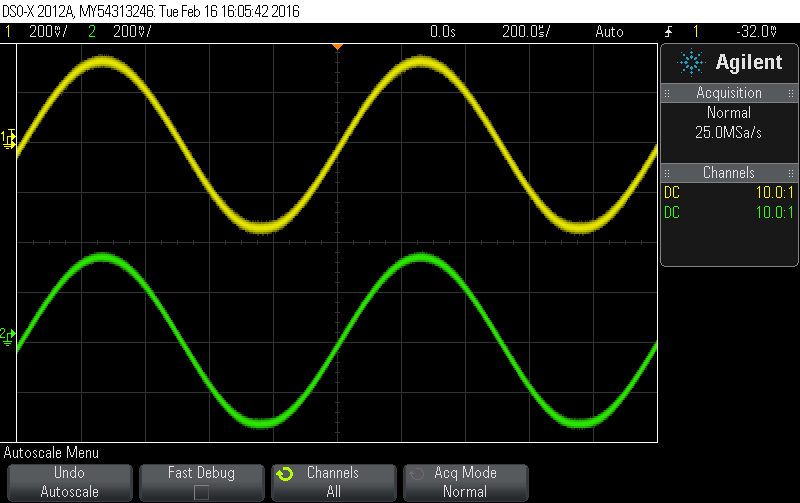
\includegraphics[width=1\linewidth]{LabOne/AC_MeasurementTwo}
\end{center}
\caption{Oscilloscope Measurement of V$_{R1}$ (both probes connected to the same point before resistance, measured to 0V Ground)}
\label{fig:AC_OsciR1}
\end{figure}



\subexperiment{Summary}



%----------------------------------------------------------------------------------------
